% Paper template for TAR 2022
% (C) 2014 Jan Šnajder, Goran Glavaš, Domagoj Alagić, Mladen Karan
% TakeLab, FER

\documentclass[10pt, a4paper]{article}

\usepackage{tar2023}

\usepackage[utf8]{inputenc}
\usepackage[pdftex]{graphicx}
\usepackage{booktabs}
\usepackage{amsmath}
\usepackage{amssymb}

\title{Well, some find it funny: Exploring alternative methods of combining Humicroedit annotator scores}

\name{Dorijan Cirkveni} 

\address{
University of Zagreb, Faculty of Electrical Engineering and Computing\\
Unska 3, 10000 Zagreb, Croatia\\ 
\texttt{dc50155@fer.hr}\\
}
          
         
\abstract{
Humor is an inherently subjective matter, as can be seen in the Humicroedit dataset's annotator grades which diverge greatly for higher averages, which this paper suggests might require an annotation analysis method different than those traditionally used on high-agreement datasets. In order to achieve a more evenly distributed labeling system, this paper tests a variety of annotator weights and a variety of methods to determine the ideal set of weights, and then compares performance on dataset with the regular mean.
}

\begin{document}

\maketitleabstract

\section{Introduction}
\label{sec:intro}

Artificial intelligence has been making major strides recently both in terms of development and practical usage, especially with the advent of LLMs such as ChatGPT as well as stable diffusion models such as Midjourney. However, certain tasks still remain outside its grasp. 

One such task is the detection, analysis, and generation of humor, a task that continues to elude the methods used. And unlike humor recognition (Khodak et al., 2017; Davidov et al., 2010; Barbieri and Saggion, 2014; Reyes et al., 2012; Cattle and Ma, 2018; Bertero and Fung, 2016; Yang et al., 2015), humor generation using artificial intelligence has proven especially tasking. One obstacle in this line of research is the scarcity of public datasets, and even greater scarcity - if not outright absence - of topic-appropriate public datasets.

One large problem in this field of study is bias, because humor is as subjective as it is complex which makes it significantly challenging to tackle from a natural language analysis/synthesis standpoint.

There are two common approaches to this problem in terms of reducing domain size and therefore annotator bias, one being to focus on a specific domain (TODO: insert citations) and the other being to focus on a specific research topic.

The underlying paper of this paper, \textit{“President Vows to Cut Taxes Hair”:
Dataset and Analysis of Creative Text Editing for Humorous Headlines} (Hossain et al., 2019), provides one dataset that is an example of the latter. A lot of care was put into eliminating annotator bias. However, as this paper suggests, these efforts might prove futile as humor is an inherently subjective activity unsuitable for such approaches.

In particular, this paper suggests alternative approaches to arithmetic mean when combining annotator grades, such as only considering top 2 grades or assigning custom weights to annotator scores.

\section{Related Work}
Alongside Humicroedit, there are other works such as A Large Self-Annotated Corpus for Sarcasm (Khodak et al., 2017), with a corpus that makes Humicroedit pale in comparison (1.3 million sarcastic statements - 10 times more than any previous dataset - and many times more instances of non-sarcastic statements),
Semi-Supervised Recognition of Sarcastic Sentences in Twitter and Amazon, and Modelling Sarcasm in Twitter, a Novel Approach. However, this paper focuses entirely on Humicroedit and its attempt to curb annotator bias.


\section{Humicroedit annotation methods}

The Humicroedit dataset includes a list of 5, 10, or 15 annotator scores, with a vast majority only having 5 scores. However, a more manageable featureset was provided alongside it, featuring 5 annotator scores for every entry. These scores are integers from 0 to 3, and they are sorted in ascending order.

Unfortunately, these annotator sets do not appear to connect to individual annotators, making it difficult to model annotator profiles.

\subsection{Annotation data properties}
 
As mentioned in~\ref{sec:intro}, Humicroedit was designed with an intention of minimizing annotator bias.. However, as noted in the paper, despite the writers' effort of carefully qualifying annotators, their perception of headlines in regards of humor present was influenced by their knowledge, preferences, bias and stance towards information presented in the headlines.

\begin{figure}
\begin{center}
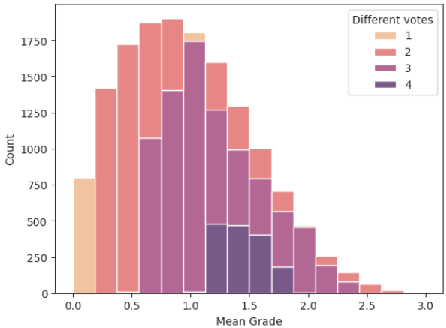
\includegraphics[width=\columnwidth]{vote distribution.pdf}
\caption{Distribution of votes for entire dataset.}
\label{fig:figure1}
\end{center}
\end{figure}

This bias is best seen in the annotator vote distribution, as lower mean scores are closer to unanimous than higher mean scores (as well as more common) as seen in Figure~\ref{fig:figure1}.


Annotator bias may also be presenting itself in topic frequency, as seen by one topic that appears in dataset entries more often than any other, as seen in Figure~\ref{fig:figure2} at 39 percent of the total dataset size.

\begin{figure}
\begin{center}
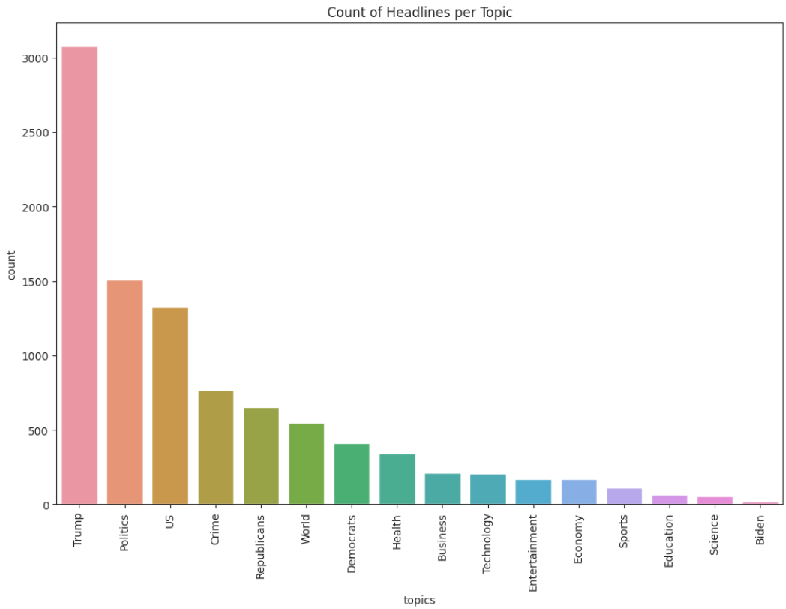
\includegraphics[width=\columnwidth]{topics_disproportion.pdf}
\caption{As we can see on this chart, a disproportionate amount of headline edits has been written on the topic of Donald J. Trump, a notable and controversial media personality and then-incumbent (45th) president of the United States of America.}
\label{fig:figure2}
\end{center}
\end{figure}



\section{Distribution measurement methods}
In order to effectively choose our weights, visual confirmation will not be a sufficient measure.
In this paper we shall use 4 different methods of determining how even is the label distribution: the Chi-Square uniformity test, the Cramér-von Mises uniformity test, and a custom uniformity test developed specifically for this purpose.
\subsection{Custom uniformity test}
The custom uniformity test is based on the method we used to display unevenly wide histogram bars:

\begin{enumerate}
\item n is the number of unique values, and the number of bars. $x_i$ is value of unique value i, and $y_i$ is its frequency.

\item Set up limits between unique values to their arithmetic mean,

\begin{equation}\label{eq:bars}
lim_i = (x_i + x_i+1)/2, i>0,i<n
\end{equation}

\item Set up beginning and end limits in a way that first and last bars are centered on their values
\begin{equation}\label{eq:lim_0}
lim_0 = x_0*2 - lim_1
\end{equation}
\begin{equation}\label{eq:lim_n}
lim_n = x_n*2 - lim_n-1
\end{equation}

\item Calculate densities of data for each bar:
\begin{equation}\label{eq:lim_n}
d_i = y_i/(lim_i+1 - lim_i) i>=0,i<n
\end{equation}

\item Calculate reference density (for perfect set):
\begin{equation}\label{eq:lim_n}
d_{total} = y/(lim_n - lim_0)
\end{equation}

\item Apply weighted square mean error:
\begin{equation}\label{eq:lim_n}
sme = \sum_{i=1}^n (lim_i+1 - lim_i)*(d_i-d_{total})^2
\end{equation}


\item Divide result by reference density square:
\begin{equation}\label{eq:lim_n}
sme_{adjusted} = sme/(lim_i+1 - lim_i)*d_{total}^2
\end{equation}
\end{enumerate}

\subsection{Unweighted arithmetic mean (reference values)}

\begin{table}
\caption{Using methods on standard mean}
\label{tab:t1}
\begin{center}
\begin{tabular}{ll}
\toprule
Method & Result \\
\midrule
Custom Uniformity & 4.350 \\
Chi Square Uniformity & 5114.936 \\
Cramér-von Mises Uniformity & 1056.477 \\
\bottomrule
\end{tabular}
\end{center}
\end{table}
First, we will determine the base distribution values by testing them on the provided labels, and the results of this are visible in Table~\ref{tab:t1}.

These values will be useful once we compare the alternative methods to them.

\section{Alternatives to simple aritmethic mean}
\subsection{Masking some of the annotator scores}
\begin{table}[ht]
\centering
\caption{Custom uniformity}
\begin{tabular}{|c|c|}
\hline
Data & Score \\
\hline
$[0, 0, 0, 0, 1]$ & 0.088 \\
$[0, 0, 0, 1, 1]$ & 0.340 \\
$[0, 0, 1, 1, 1]$ & 1.073 \\
$[0, 1, 1, 1, 1]$ & 2.366 \\
$[1, 1, 1, 1, 1]$ & 4.350 \\
\hline
\end{tabular}
\label{tab:custom-uniformity}
\end{table}

\begin{table}[ht]
\centering
\caption{Chi-Square uniformity}
\begin{tabular}{|c|c|}
\hline
Data & Score \\
\hline
$[0, 0, 0, 1, 0]$ & 529.4771 \\
$[0, 1, 0, 0, 1]$ & 79.147 \\
$[0, 0, 1, 1, 1]$ & 268.462 \\
$[0, 1, 1, 1, 1]$ & 1218.731 \\
$[1, 1, 1, 1, 1]$ & 5114.937 \\
\hline
\end{tabular}
\label{tab:chi-square-uniformity}
\end{table}

\begin{table}[ht]
\centering
\caption{Cramer-Von Mises uniformity}
\begin{tabular}{|c|c|}
\hline
Data & Score \\
\hline
$[0, 0, 1, 0, 0]$ & 1443.005 \\
$[1, 0, 1, 0, 0]$ & 461.433 \\
$[1, 1, 0, 1, 0]$ & 238.483 \\
$[1, 1, 1, 1, 0]$ & 280.723 \\
$[1, 1, 1, 1, 1]$ & 1056.477 \\
\hline
\end{tabular}
\label{tab:cramer-von-mises-uniformity}
\end{table}

First, we are going to use simple masking by only using certain annotator scores. Score masks are denoted as follows:
$[0,1,0,1,0]$, 0 and 1 used to mark ignored and considered scores respectively.

In this test, 31 ($2^5 -1 $) possible combinations are tested, sorted by result, divided into groups by number of scores used, and best result of each group is displayed, as lower number of annotator scores used may lead to less reliable results.

In Table~\ref{tab:custom-uniformity}, we can see the custom method produced more/less expected  results, which is to say the highest annotator scores proved to provide the most uniform results.

However, Tables ~\ref{tab:chi-square-uniformity} and ~\ref{tab:cramer-von-mises-uniformity} tell a different story as not only do their scores give better scores for multiple annotators, 
\section{Future work}
Unfortunately, due to time limitations brought upon by unfortunate circumstances and poor planning, we were unable to completely explore this topic. Future work in this line of reseach may involve further optimization of annotator grade weights towards providing more uniform results.
Further work extending on this paper should involve testing in [-1,1] domain using various optimization methods.

However, we recommend that future studies, instead of attempting to stifle subjectivity in humor recongnition, embrace the inherently subjective nature of humor through methods such as pseudonymous annotator ID in data collection which could facilitate this process.



\section{Referencing literature}

Hossain, Nabil; Krumm, John; Gamon, Michael: “President Vows to Cut Taxes Hair”: Dataset and Analysis of Creative Text Editing for Humorous Headlines

Khodak, Mikhail; Saunshi, Nikunj; Vodrahalli, Kiran: A Large Self-Annotated Corpus for Sarcasm

Davidov, Dmitry; Tsur, Oren; Rappoport, Ari: Semi-supervised recognition of sarcasm in Twitter and Amazon

Barbieri, Francesco; Saggion, Horacio; Ronzano, Francesco: Modelling sarcasm in twitter, a novel approach

Reyes, Antonio; Rosso, Paolo; Buscaldi, Davide: From humor recognition to irony detection: The figurative language of social media

\section{Conclusion}

Humor is one of the tasks that artificial intelligence has the most difficulty in, which is a task made even more difficult by the lack of available datasets. Humicroedit is one of the attempts to provide such a dataset. However, there may be issues with the approach taken by it.

This paper attempted to find a way to acknowledge the inherent subjectivity by assigning weights to annotator scores and evaluating the distributions of resulting labels. Unfortunately, only a basic {0,1} weight domain was tested in this paper, with 31 possible weight sets being tested.

Further work extending on this paper should involve testing in [-1,1] domain using various optimization methods, while future work in the field should, instead of attempting to stifle subjectivity in humor recongnition, embrace the inherently subjective nature of humor through methods such as pseudonymous annotator ID in data collection which could facilitate this process.

\section*{Acknowledgements}

I would like to thank Gabriel Marinković for helping me try to make this paper.

\bibliographystyle{tar2023}
\bibliography{tar2023} 

\end{document}

